\documentclass{beamer}
\usepackage{hyperref}
\usepackage{listings}
\usepackage{graphicx}
\usepackage{upquote}
\usepackage{textcomp}

\usepackage[T1]{fontenc}
\usepackage[utf8]{inputenc}

\usepackage{DejaVuSansMono}

\lstset{basicstyle=\fontfamily{dejavu}\footnotesize\ttfamily,breaklines=true}
\lstset{frame=bottomline}
\lstset{upquote=true}

\usetheme{Rochester}
\title{ Git and You <3 } 
\subtitle{(Working Title)}
\author{Andrew Ballinger}
\begin{document}

\frame{\titlepage}

\begin{frame}[fragile]
\frametitle{What is a git and how do I get one?}
Git is a version control system developed for working on the Linux Kernel.

\vspace{1em}

\begin{lstlisting}[frame=single]
 git init
 ls
 ls .git
 git status
\end{lstlisting}

\end{frame}

\begin{frame}[fragile]
\frametitle{Tracking files}

Lets add some files.

\vspace{1em}

\begin{lstlisting}[frame=single]
 touch some_random_file
 echo "puts 'Hello World'" > hello.rb
 ruby hello.rb
 git add hello.rb
 git status
\end{lstlisting}

\vspace{1em}

\begin{lstlisting}[frame=single]
echo "some_random_file" >> .gitignore
git status
\end{lstlisting}

\end{frame}

\begin{frame}[fragile]
\frametitle{Tracking changes}

Lets save this stuff.

\vspace{1em}

\begin{lstlisting}[frame=single]
  git commit -m "This is the first commit"
  git status
  git log
\end{lstlisting}

\begin{figure}[p]
  \centering
  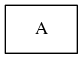
\includegraphics[height=5em]{first_commit.png}
  \caption{First commit}
\end{figure}

\end{frame}

\begin{frame}[fragile]
\frametitle{Tracking changes}

Lets do some stuff.

\vspace{1em}

\begin{lstlisting}[frame=single]
  echo "puts 'Hello Fish'" > hello.rb
  ruby hello.rb
  git commit -m 'Hello Fish?'
  echo 'puts "Hello " + [0x1F431].pack("U*")' > hello.rb
  git commit -am 'Hello ?'
  ruby hello.rb
\end{lstlisting}

\begin{figure}[p]
  \centering
  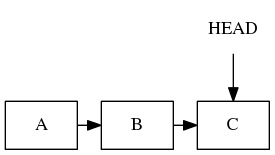
\includegraphics[height=5em]{some_commits.png}
\end{figure}

\end{frame}

\begin{frame}[fragile]
\frametitle{What is HEAD?}

Spoiler: It's the current commit

\vspace{1em}

\begin{lstlisting}[frame=single]
  git checkout HEAD~1
  ruby hello.rb
\end{lstlisting}

\begin{figure}[p]
  \centering
  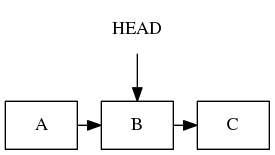
\includegraphics[height=5em]{head.png}
\end{figure}

\end{frame}

\begin{frame}[fragile]
\frametitle{Branching}

\begin{lstlisting}[frame=single]
  git branch "fish_rule"
  git checkout "fish_rule"
  echo 'puts "Fish Rule"' >> hello.rb
  ruby hello.rb
  git commit -am "Fish are way better then cats"
  echo '["Fish live in the ocean."]' >> fish_facts.json
  git add fish_facts.json
  git commit -am "Some fish facts"
  git log
\end{lstlisting}

\begin{figure}[p]
  \centering
  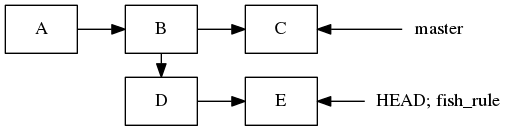
\includegraphics[height=5em]{fish.png}
\end{figure}

\end{frame}

\begin{frame}[fragile]
\frametitle{Merging}

Merging allows you to combine changes

\vspace{1em}

\begin{lstlisting}[frame=single]
  git diff master
  git merge master
\end{lstlisting}

\vspace{1em}

O noes! Some compromise must be reached

\vspace{1em}

\begin{lstlisting}[frame=single]
  git status
  git checkout --ours hello.rb 
  git status
  git commit -am "Fish are better"
  git status
\end{lstlisting}

\begin{figure}[p]
  \centering
  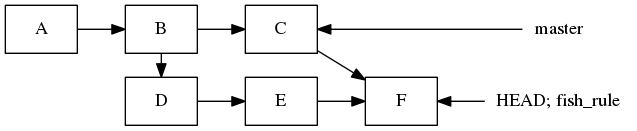
\includegraphics[height=5em]{merge.png}
\end{figure}

\end{frame}

\begin{frame}[fragile]
\frametitle{Fast Forwarding}

Fish are super awesome, they're going into production.

\vspace{1em}

\begin{lstlisting}[frame=single]
 git checkout master
 git merge fish_rule
 git status
 git log
\end{lstlisting}

\begin{figure}[p]
  \centering
  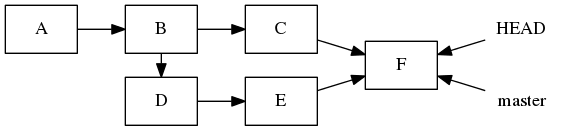
\includegraphics[height=5em]{fast_forward.png}
\end{figure}

\end{frame}

\begin{frame}[fragile]
\frametitle{Push and Pull}

Push moves your current branch onto a remote server

\vspace{1em}

\begin{lstlisting}[frame=single]
  git push 
\end{lstlisting}

\vspace{1em}

Pull gets (merges!) your current branch from the remote server

\vspace{1em}

\begin{lstlisting}[frame=single]
  git pull 
\end{lstlisting}

\end{frame}

\begin{frame}

\frametitle{That's it (basically)}

\begin{figure}[p]
  \centering
  
\includegraphics[height=15em]{howard.jpg}
  \caption{Sure sure, you can use git, but can you really use git?}
\end{figure}

\end{frame}



\begin{frame}
\frametitle{Resources}

\begin{itemize}
\item{githug}
\end{itemize}
  
\end{frame}

\end{document}
